\sect{Nuestro acercamiento}

Sea $P$ un número natural arbitrario, considere la función sobre $\mathbb{R^+}$ , $f(x) = x^P$, la cual tiene una forma similar a la siguiente, cuando $P > 1$

\definecolor{col_na_0}{HTML}{008080}
\begin{center}
    \begin{tikzpicture}
        \begin{axis}[
            xmin=-0.5,
            xmax=5,
            ymin=-0.5,
            ymax=25,
            axis lines=center,
            xlabel=$X$,
            ylabel=$Y$,
            ticks=none,
            x label style={at={(axis description cs: 1.1, -0.03)}},
            y label style={at={(axis description cs: 0.03, 1.1)}},
            clip=false,
        ]
            \addplot[color=col_na_0, samples=100, domain=0:4.5]{x^2}
            node[right, pos=1]{$f(x) = x^P$};
        \end{axis}
    \end{tikzpicture}
\end{center}

Sea $n$ un número natural, se puede pensar de la suma $\displaystyle\sum_{k=1}^{n}k^P$ como una aproximación a $\displaystyle\int_{0}^{n}x^P dx$

Tomemos la última parte de esta aproximación:

\definecolor{col_na_1}{HTML}{FFDAB9}
\definecolor{col_na_2}{HTML}{E0FFFF}
\begin{center}
    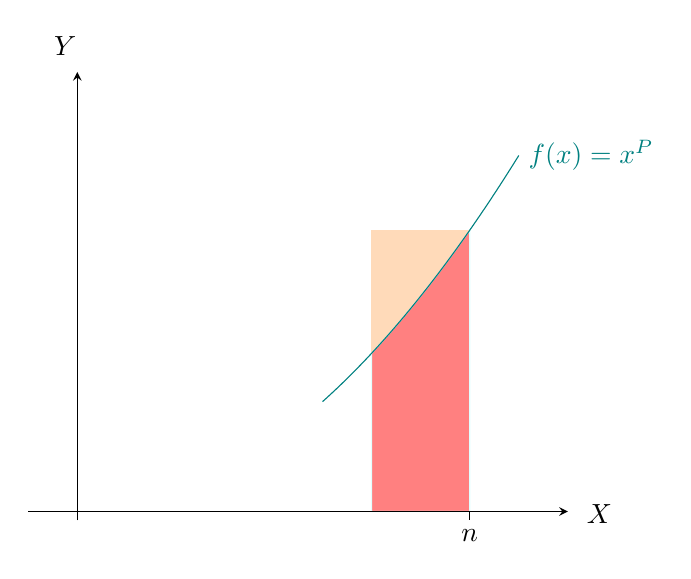
\begin{tikzpicture}
        \begin{axis}[
            xmin=-0.5,
            xmax=5,
            ymin=-0.5,
            ymax=25,
            axis lines=center,
            xlabel=$X$,
            ylabel=$Y$,
            ticks=none,
            x label style={at={(axis description cs: 1.1, -0.03)}},
            y label style={at={(axis description cs: 0.03, 1.1)}},
            clip=false,
            axis on top=true,
        ]
            \filldraw[color=col_na_1] (3, 16) rectangle (4,0);
            \addplot[color=col_na_2, samples=100,domain=3:4, fill=red!50]{x^2}\closedcycle;
            \addplot[color=col_na_0, samples=100, domain=2.5:4.5,]{x^2}
            node[right, pos=1]{$f(x) = x^P$};
            \draw (4, 0) -- (4, -0.5) node[anchor=north]{$n$};
        \end{axis}
    \end{tikzpicture}
\end{center}

Considerando el restante del área del rectángulo ($A$) con respecto al área bajo la curva como $R(n)$ se tiene la siguiente igualdad.

\[A = R(n) + \int_{n-1}^{n}x^P dx\]

Si se piensa en la suma, en este caso, $A$ representa el sumatorio desde $n-1$ hasta $n$, por lo que al definir $R$ en función de cada natural hasta $n$ se puede descomponer la suma en otra suma.
